% =====================================================================
%  Capítulo 11 — Resolução numérica
%  Inserir depois da seção "Testes clássicos".
% =====================================================================
\section{Resolução numérica}
\label{sec:cap11-numerica}

Três resultados deste capítulo foram enunciados sem conta explícita: o valor
da ISCO, a precessão do periélio e o comportamento do tempo coordenado perto
do horizonte. Nenhum deles é acessível por integração em forma fechada
elementar, e é justamente aí que o cálculo numérico deixa de ser ilustração e
passa a ser método. Esta seção resolve os três, valida cada resultado contra
um limite conhecido e produz as figuras usadas nas seções anteriores. Os
scripts completos estão em \texttt{codigo/}; aqui reproduzimos apenas os
trechos que carregam a física.

Trabalhamos com $G = c = 1$ e $M = 1$, de modo que $r$ é medido em massas
gravitacionais: $r = 6$ significa $r = 6GM/c^2$. Para uma partícula massiva
no plano equatorial, com $E$ e $L$ conservados por unidade de massa de
repouso,
\begin{equation}
  \left(\rd{r}{\tau}\right)^{2} = E^{2} - \Veff(r),
  \qquad
  \Veff(r) = \left(1 - \frac{2M}{r}\right)\left(1 + \frac{L^{2}}{r^{2}}\right).
  \label{eq:cap11-veff}
\end{equation}

\begin{atencao}
Integrar diretamente $\dd r/\dd\tau = \pm\sqrt{E^{2}-\Veff}$ é a primeira
tentativa de quase todo mundo, e ela falha: nos pontos de retorno o radicando
passa por zero e o integrador ou trava ou escolhe o sinal errado. Derive a
equação~\eqref{eq:cap11-veff} uma vez em $\tau$ e integre a forma de segunda
ordem,
\[
  \rd{^{2}r}{\tau^{2}} = -\frac{M}{r^{2}} + \frac{L^{2}}{r^{3}}
                          - \frac{3ML^{2}}{r^{4}},
\]
que é regular nos pontos de retorno e vale exatamente, sem aproximação de
campo fraco.
\end{atencao}

\subsection{Python}

\programa[ISCO, precessão do periélio em campo forte, deflexão da luz e queda radial.]{codigo/cap11\_geodesicas\_schwarzschild.py}

\subsubsection*{Órbitas circulares e a ISCO}

Órbitas circulares são extremos de $\Veff$. A família de raios circulares sai
de $\Veff'(r)=0$, que dá $L^{2} = Mr^{2}/(r-3M)$; a ISCO é o ponto em que
mínimo e máximo se fundem, isto é, onde $\Veff''=0$ ao longo dessa família.
Isso é uma raiz unidimensional, resolvida com \texttt{brentq}.

\begin{saida}
\begin{lstlisting}[style=rgsaida]
r_ISCO (numerico) = 6.0000000000 M      (exato: 6 M)
L_ISCO            = 3.4641016151 M      (exato: sqrt(12) = 3.4641016151)
E_ISCO            = 0.9428090416        (exato: sqrt(8/9) = 0.9428090416)
eficiencia de acrecao 1 - E_ISCO = 0.057191  (5.72 % da massa de repouso)
orbita de fotons  = 3.0000000000 M      (exato: 3 M)
\end{lstlisting}
\end{saida}

\begin{central}
O número $1-E_{\rm ISCO} = 5{,}72\,\%$ não é um detalhe numérico: é a fração
da massa de repouso que um disco fino pode irradiar antes que a matéria
mergulhe no buraco negro. Compare com $\sim 0{,}7\,\%$ da fusão de hidrogênio.
Acreção em buraco negro sem rotação já é quase uma ordem de grandeza mais
eficiente que a fonte de energia das estrelas.
\end{central}

\subsubsection*{Precessão do periélio}

Com $p$ (semi-latus rectum) e $e$ dados, as constantes de movimento ficam
determinadas, e o periélio ocorre sempre que $\dot r$ muda de sinal de
negativo para positivo. Localizamos esses instantes por interpolação linear e
medimos a diferença azimutal entre periélios consecutivos.

\begin{saida}
\begin{lstlisting}[style=rgsaida]
Delta phi por orbita, numerico = 1.231264 rad
Delta phi por orbita, 6 pi M/p = 0.942478 rad
exato para e -> 0: 2 pi [(1-6M/p)^(-1/2) - 1] = 1.226658 rad

  p/M      numerico        6 pi M/p      razao
    20   1.231264e+00   9.424778e-01     1.3064
    50   4.151280e-01   3.769911e-01     1.1012
   200   9.644314e-02   9.424778e-02     1.0233
  1000   1.893557e-02   1.884956e-02     1.0046

Mercurio: 5.0187e-07 rad/orbita  ->  42.98 arcsec/seculo
\end{lstlisting}
\end{saida}

Vale examinar essa saída com cuidado, porque ela contém três lições
diferentes. Primeiro, em $p = 20M$ a fórmula $6\pi M/p$ erra por $31\,\%$:
ela é apenas o termo de primeira ordem de uma série em $M/p$, e o campo ali
não é fraco. Segundo, a última coluna mostra a razão tendendo a~$1$ conforme
$p$ cresce --- é assim que se verifica que uma aproximação está sendo usada
dentro do seu domínio de validade. Terceiro, o valor numérico $1{,}2313$ para
$e = 0{,}4$ está próximo do resultado exato $1{,}2267$ obtido adiante para
órbitas quase circulares; a diferença é o efeito da excentricidade, de ordem
$e^{2}$.

E, ao fim, o mesmo código aplicado a Mercúrio devolve os $42{,}98''$ por
século que Einstein calculou em novembro de 1915 --- o primeiro número que a
teoria acertou.

\begin{figure}[htbp]
  \centering
  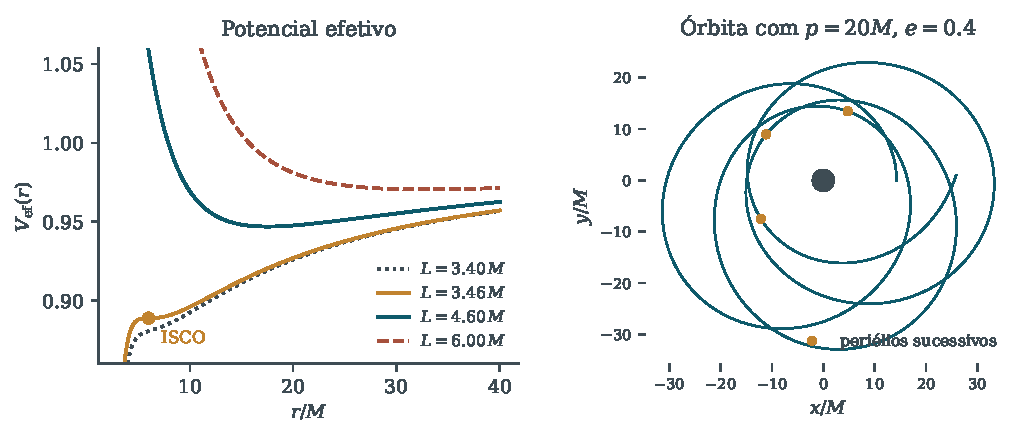
\includegraphics[width=\linewidth]{figuras/cap11_potencial_orbita.pdf}
  \caption{À esquerda, o potencial efetivo~\eqref{eq:cap11-veff} para vários
  valores de $L$. Abaixo de $L = \sqrt{12}\,M$ o poço desaparece e não há
  órbita ligada; o ponto de inflexão marca a ISCO. À direita, a órbita
  integrada com $p = 20M$ e $e = 0{,}4$: os periélios sucessivos (em âmbar)
  não se repetem no mesmo ângulo, e a órbita não fecha. O disco central é o
  horizonte.}
  \label{fig:cap11-potencial}
\end{figure}

\subsubsection*{Deflexão da luz}

Para geodésicas nulas convém trocar de variável para $u = 1/r$ e usar $\phi$
como parâmetro, o que transforma o problema em
$u'' + u = 3Mu^{2}$. O raio vem do infinito ($u=0$), passa pelo periastro e
volta ao infinito; o evento de retorno a $u = 0$ é detectado pelo próprio
integrador.

\begin{saida}
\begin{lstlisting}[style=rgsaida]
     b/M     numerico         4M/b   + 15 pi M^2/(4b^2)
      10 5.903958e-01 4.000000e-01         5.178097e-01
      50 8.508345e-02 8.000000e-02         8.471239e-02
     200 2.029997e-02 2.000000e-02         2.029452e-02
    1000 4.011823e-03 4.000000e-03         4.011781e-03

borda do Sol: 1.751 arcsec
\end{lstlisting}
\end{saida}

A terceira coluna inclui a correção de segunda ordem. Note como ela recupera
quase todo o erro em $b = 50M$ e praticamente todo em $b \geq 200M$, mas
ainda falha em $b = 10M$: perto da órbita de fótons nenhuma expansão em $M/b$
sobrevive.

\subsubsection*{Queda radial e a divergência do tempo coordenado}

\begin{saida}
\begin{lstlisting}[style=rgsaida]
tempo proprio ate' o horizonte  = 33.700870 M
tempo proprio ate' r = 0        = 35.124074 M
  ate' r =  3.000 M :  tau =   32.4099 M   t =      40.9383 M
  ate' r =  2.100 M :  tau =   33.5873 M   t =      47.1540 M
  ate' r =  2.010 M :  tau =   33.6897 M   t =      51.9068 M
  ate' r =  2.001 M :  tau =   33.6998 M   t =      56.5266 M
\end{lstlisting}
\end{saida}

Esta é a tabela mais eloquente do capítulo. A cada fator de dez que
aproximamos o alvo do horizonte, o tempo próprio muda na quarta casa decimal
--- a queda está praticamente terminada --- enquanto o tempo coordenado sobe
mais cinco unidades de $M$, sem sinal de parar. A divergência é logarítmica,
e o observador em queda não sente absolutamente nada de especial ao cruzar
$r = 2M$.

\begin{figure}[htbp]
  \centering
  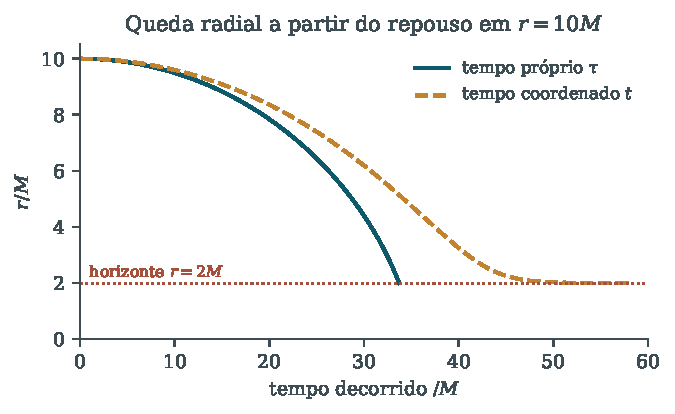
\includegraphics[width=0.72\linewidth]{figuras/cap11_queda_radial.pdf}
  \caption{Queda radial a partir do repouso em $r = 10M$. Em tempo próprio a
  trajetória cruza o horizonte e chega a $r=0$ em tempo finito; em tempo
  coordenado ela se acumula assintoticamente sobre $r = 2M$. As duas curvas
  descrevem a mesma queda, medida por relógios diferentes.}
  \label{fig:cap11-queda}
\end{figure}

\subsection{Mathematica}

\programa[Christoffel, Riemann e Ricci de Schwarzschild; Kretschmann; extração exata da ISCO e da precessão.]{codigo/cap11\_schwarzschild\_simbolico.wl}

O papel do cálculo simbólico aqui é complementar, não redundante: ele fornece
as expressões exatas contra as quais o resultado numérico é conferido. Os
símbolos de Christoffel, o tensor de Riemann e o de Ricci são construídos a
partir da métrica com as mesmas convenções de índice do
Capítulo~\ref{cap:curvatura}.

O mesmo tensor de Riemann fornece o escalar de Kretschmann,
$R_{\alpha\beta\gamma\delta}R^{\alpha\beta\gamma\delta} = 48M^{2}/r^{6}$,
citado na Seção~\ref{sec:horizonte} para separar singularidade de coordenada
de singularidade física.

A parte mais útil é a extração exata da ISCO e da precessão. Escrevendo
$q = L^{2}$, o script resolve $\partial_r\Veff=0$ para obter a família de
órbitas circulares, $q = Mr^{2}/(r-3M)$, impõe também $\partial_r^2\Veff=0$
e recupera $r=6M$, $q=12M^{2}$; em seguida compara as frequências radial e
azimutal.

O resultado é
\begin{equation}
  \Delta\phi_{\text{órbita}}
  = 2\pi\left[\left(1 - \frac{6M}{r}\right)^{-1/2} - 1\right]
  = \frac{6\pi M}{r} + \frac{27\pi M^{2}}{r^{2}} + \mathcal{O}\!\left(\frac{M^{3}}{r^{3}}\right),
  \label{eq:cap11-precessao-exata}
\end{equation}
válido no limite de órbitas quase circulares. Duas leituras: o primeiro termo
é exatamente a fórmula clássica usada para Mercúrio, e a expressão inteira
diverge em $r = 6M$ --- na ISCO a frequência de oscilação radial vai a zero,
a órbita deixa de precessar e passa a espiralar.

\begin{central}
A verificação cruzada é o produto real desta seção. O integrador devolveu
$1{,}231264$ para uma órbita com $e = 0{,}4$; a expressão
exata~\eqref{eq:cap11-precessao-exata} dá $1{,}226658$ no limite $e \to 0$; a
fórmula de primeira ordem dá $0{,}942478$. Os dois primeiros concordam em
três dígitos e discordam do terceiro por $30\,\%$. Um resultado numérico que
não é confrontado com um limite analítico conhecido não é resultado: é
palpite com casas decimais.
\end{central}

